\Problem{Arbres lògics}

\Statement

Considerem arbres lògics on cada node intern correspon a una operació lògica (AND, OR o NOT) i on les fulles corresponen a variables booleanes (paraules en minúscules). Per exemple, l'arbre següent correspon a l'expressió lògica \texttt{AND(OR(a,b),NOT(c))}:

\medskip

\begin{center}
    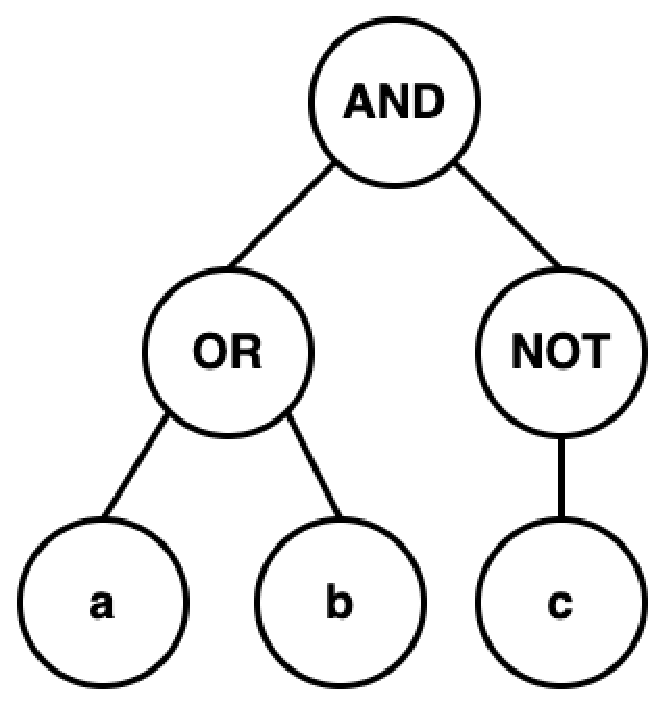
\includegraphics[width=4cm]{arbre}
\end{center}

\medskip

Les expressions lògiques s'escriuen en una línia en forma de funcions completament parantitzades, separant els paràmetres amb comes, amb els operadors en majúscules, i amb les variables en minúscules. Els operadors AND i OR tenen dues subexpressions lògiques; els operadors NOT només una. Aquests són alguns exemples d'expressions lògiques:

\begin{itemize*}
    \item \texttt{AND(OR(a,b),NOT(c))}
    \item \texttt{parell}
    \item \texttt{OR(parell,senar)}
    \item \texttt{NOT(AND(OR(a,b),AND(b,NOT(c))))}
\end{itemize*}

Avaluar un arbre lògic correspon a calcular el valor que conté la seva expressió lògica per a un conjunt de variables certes (la resta de variables es consideren falses). Per exemple, amb el conjunt de variables certes $\{\texttt{a}\}$, l'arbre de la figura s'avalua a cert, i  amb el conjunt de variables certes  $\{\texttt{c}, \texttt{a}\}$, l'arbre de la figura s'avalua a fals.

\medskip

Descarregeu-vos el codi proposat \texttt{code.cc} i completeu-lo per tal que llegeixi una expressió lògica, construeixi el seu arbre, l'escrigui, i escrigui el resultat de la seva avaluació per a diferents conjunts de variables certes (una per línia). 

\section*{Pistes}

\begin{itemize}

    \item Ja teniu molt de codi escrit, aprofiteu-lo!

    \item

Per tal de convertir un text que conté una expressió lògica a un arbre lògic, primer podeu substituir-li tots els parèntesis i comes per espais.  A continuació podeu processar en pre-ordre la seqüència de paraules resultants a través d'un \texttt{istringstream}. 

Per exemple, \texttt{AND(OR(a,b),NOT(c))} es transforma primer en \texttt{AND\textvisiblespace{}OR\textvisiblespace{}a\textvisiblespace{}b\textvisiblespace{}\textvisiblespace{}NOT\textvisiblespace{}c\textvisiblespace{}\textvisiblespace{}} i, a continuació, es processa la seva seqüència de paraules \texttt{AND}, \texttt{OR}, \texttt{a}, \texttt{b}, \texttt{NOT}, \texttt{c} a través d'un \texttt{istringstream}.  

Al \texttt{main()} teniu un exemple d'ús del \texttt{istringstream}.

\item

Evidentment, si us calen, podeu afegir noves funcions.

\item

Cap al final de la funció \texttt{main()} falta un detallet...

\end{itemize}


\SampleTwoCol


